\section{Motion Law}

	This section documents the procedure followed to generate a motion law for
	the found path. The proposed method can be used to ensure adherence to
	velocity and acceleration constraints of the actuators. Since the cable
	velocities are directly related to the actuator velocities, the motion law
	is constructed in cable space. The cable velocities $\dot{\cablevec}$ are
	related to the path $\pathsym$ through:

	\begin{equation}
		\dot{\cablevec} = \invgeometricmodel
							\left(
								\frac
								{
									\der \pathsym
								}
								{
									\der \timenorm
								}
							\right)
	\end{equation}

	A motion law

	\begin{equation}
		\motionlaw : \timesym \in \Re \mapsto \timenorm \in [0, 1]
	\end{equation}

	is now built and used to create a trajectory $\traj$ from the
	path $\pathsym$ according to:

	\begin{equation}
		\traj = \pathsym(\motionlaw(\timesym))
	\end{equation}

	This is done by finding the time ranges $\range$ where $\dot{\cablevec} >
	\dot{\cablevec}_{\max}$ or $\ddot{\cablevec} > \ddot{\cablevec}_{\max}$. Let
	$\setofranges$ be the set of such ranges. $\motionlaw$ is then constructed
	such that:

	\begin{equation}
		\frac
		{
			\motionlaw
		}
		{
			\timenorm
		}
		=
		\begin{cases}
			1,			&\timenorm \not\in \setofranges\\
			\gain_i,	&\timenorm \in \range_i \in \setofranges
		\end{cases}
		\label{eq:motion_law_construction}
	\end{equation}

	Here, $\gain_i$ is chosen such that:

	\begin{equation}
		\begin{cases}
			|\dot{\cablevec}| \leq \dot{\cablevec}_{\max}\\
			|\ddot{\cablevec}| \leq \ddot{\cablevec}_{\max}\\
		\end{cases}
			\forall\timenorm\in\range_i
	\end{equation}

	The aim of using a piecewise function such as that in
	Equation~\ref{eq:motion_law_construction} is to slow down only regions of
	the trajectory that exceed constraints instead of slowing down the entire
	trajectory. However, loss of differentiability in the motion law leads to
	decreases in the degree of continuity of the final trajectory. For this
	reason, the motion law built from Equation~\ref{eq:motion_law_construction}
	may be smoothed with B-spline curves. A B-spline of degree 2 will ensure a
	smooth velocity profile, whereas higher degree B-splines can ensure further
	degrees of continuity.

	Figure~\ref{fig:motion_law_deg1} shows the output of a planning problem
	applying Equation~\ref{eq:motion_law_construction} directly without using
	B-Splines. The top graph shows the cable lengths over time. The middle graph
	shows their velocities and the bottom graph shows the motion law. Note the
	jump steps in velocity where the slope of the motion law changes.

		\begin{figure}[hb]
			\begin{minipage}{0.5\columnwidth}
				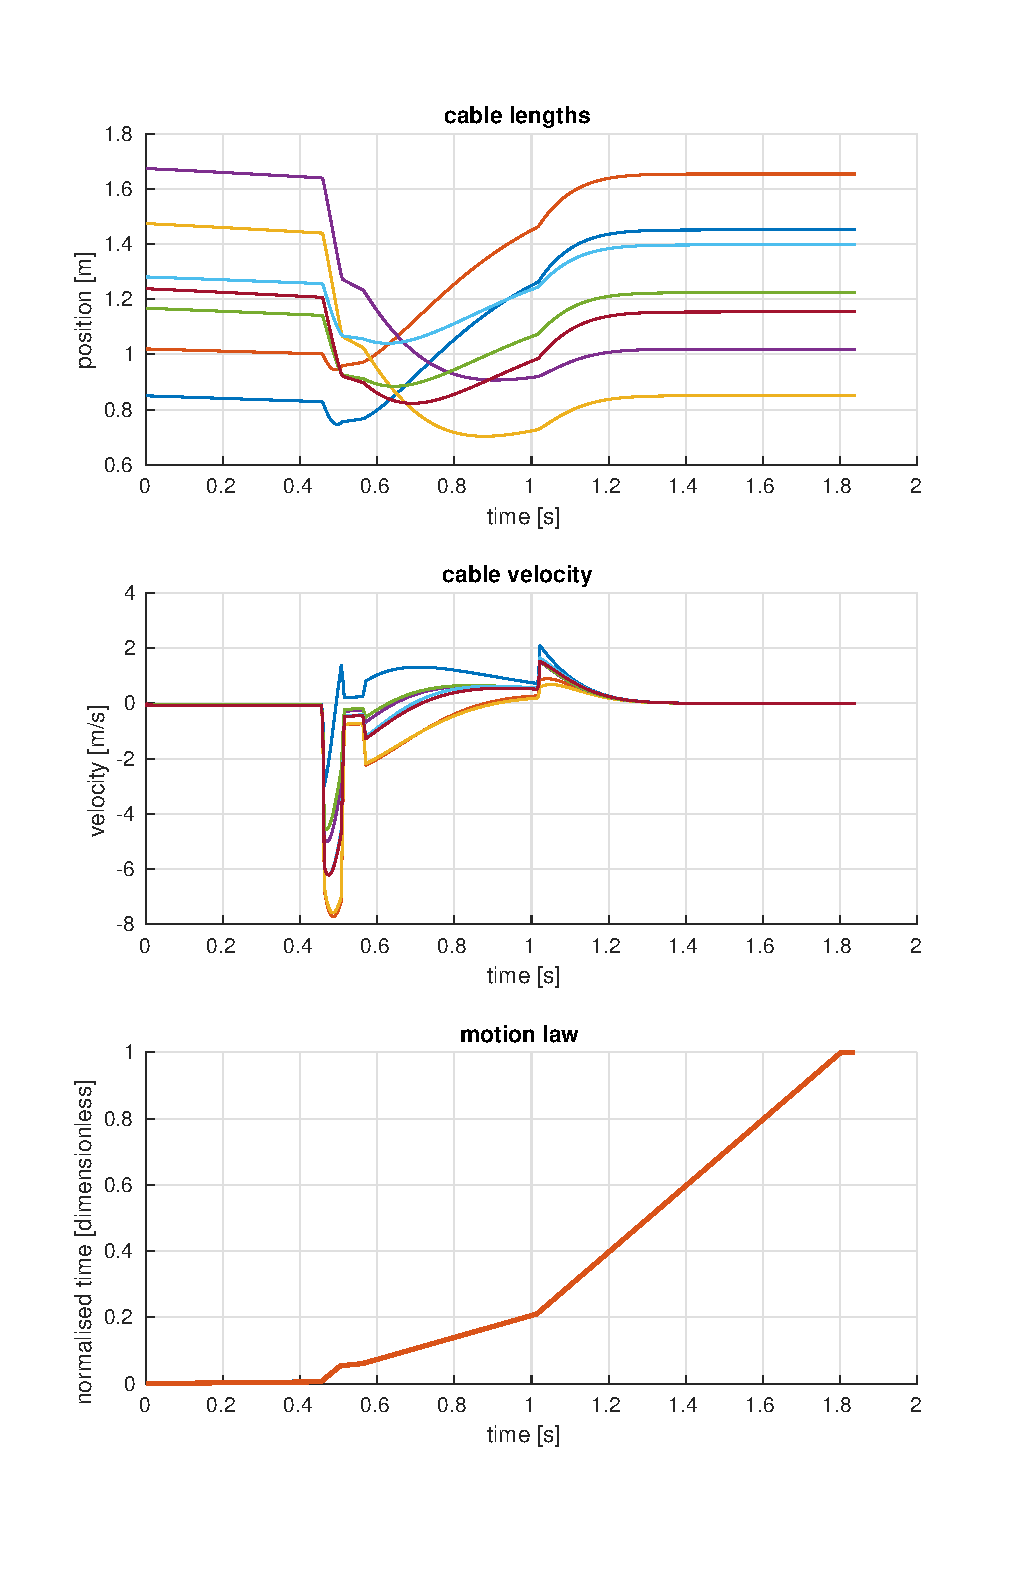
\includegraphics[width=\textwidth]{motion_law_deg_1}
				\caption{Motion Law without\\\hspace{\textwidh} B-Spline}
				\label{fig:motion_law_deg1}
			\end{minipage}%
			\begin{minipage}{0.5\columnwidth}
				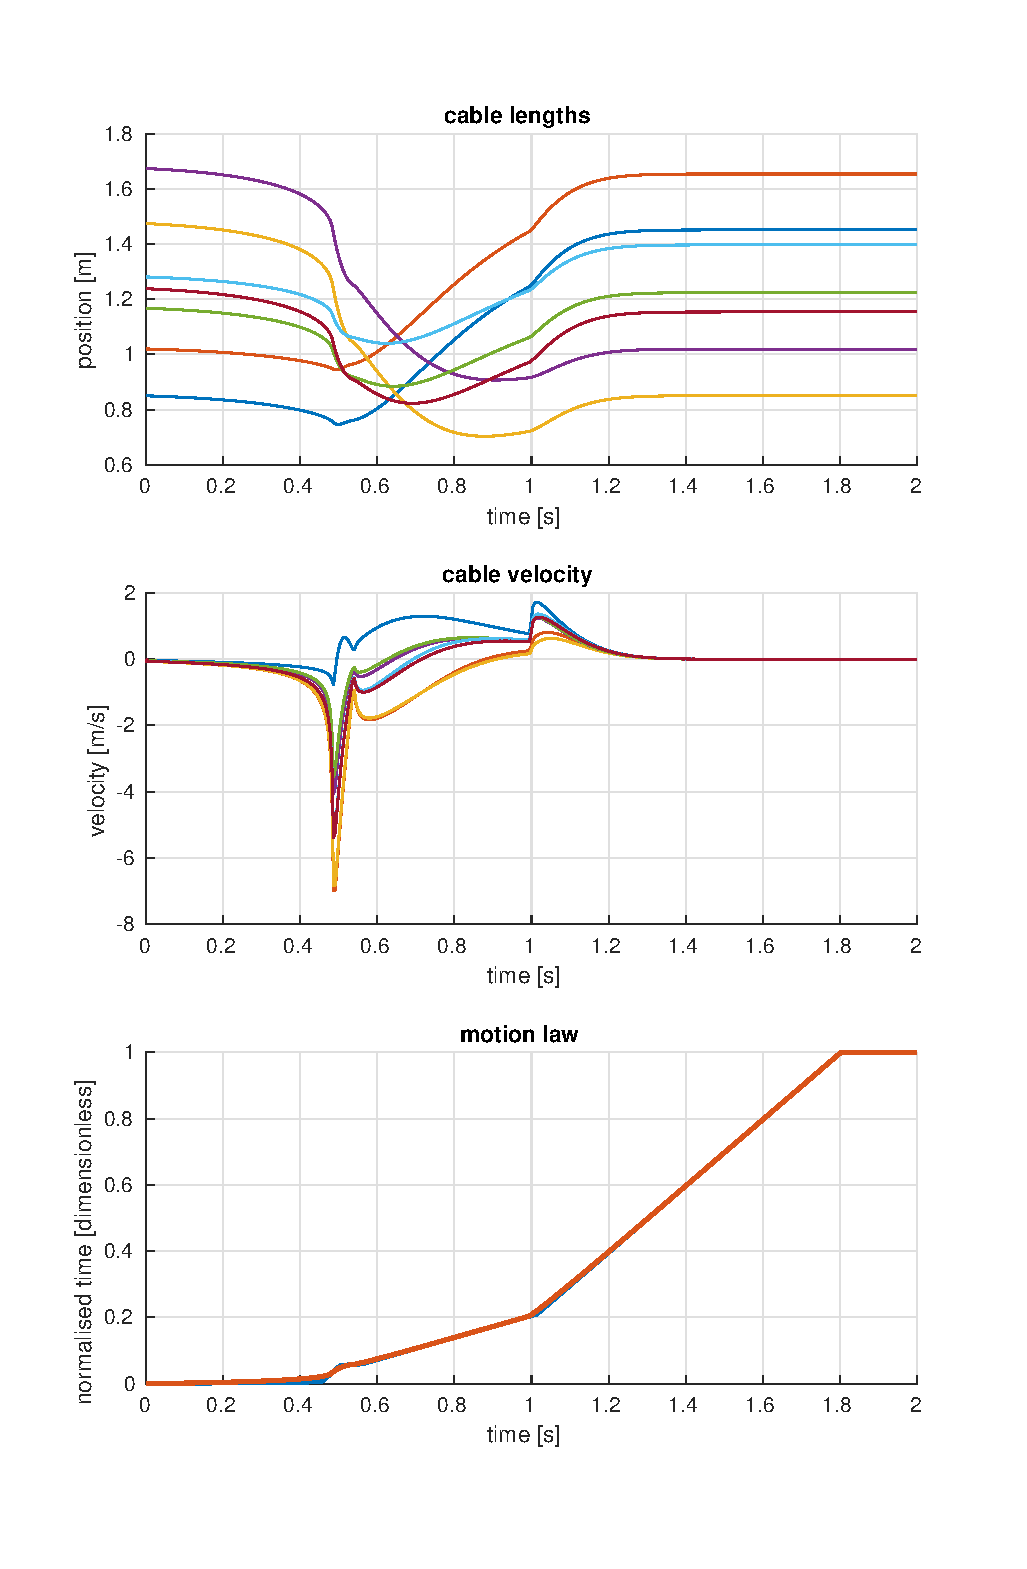
\includegraphics[width=\columnwidth]{motion_law_deg_2}
				\caption{Motion Law with B-Spline\\\hspace{\textwidth} of Degree 2}
				\label{fig:motion_law_deg2}
			\end{minipage}
		\end{figure}

	Figure~\ref{fig:motion_law_deg2} shows the effect of interpolating the
	motion law with a B-spline of degree 2. Notice how the motion law is very
	close to its original shape, but the cable length profile is now smooth.

	Figure~\ref{fig:motion_law_deg3} shows that the cable-space trajectories are
	further smoothed by using a B-spline of third degree. Finally,
	Figure~\ref{fig:motion_law_deg7} shows that very smooth profiles may be
	obtained by using higher degree splines. Note in this figure that higher
	degree splines have the tendency to depart more from the original motion
	law. This can be seen in the bottom of Figure~\ref{fig:motion_law_deg7}.

	\begin{figure}[ht]
		\begin{minipage}{0.5\columnwidth}
			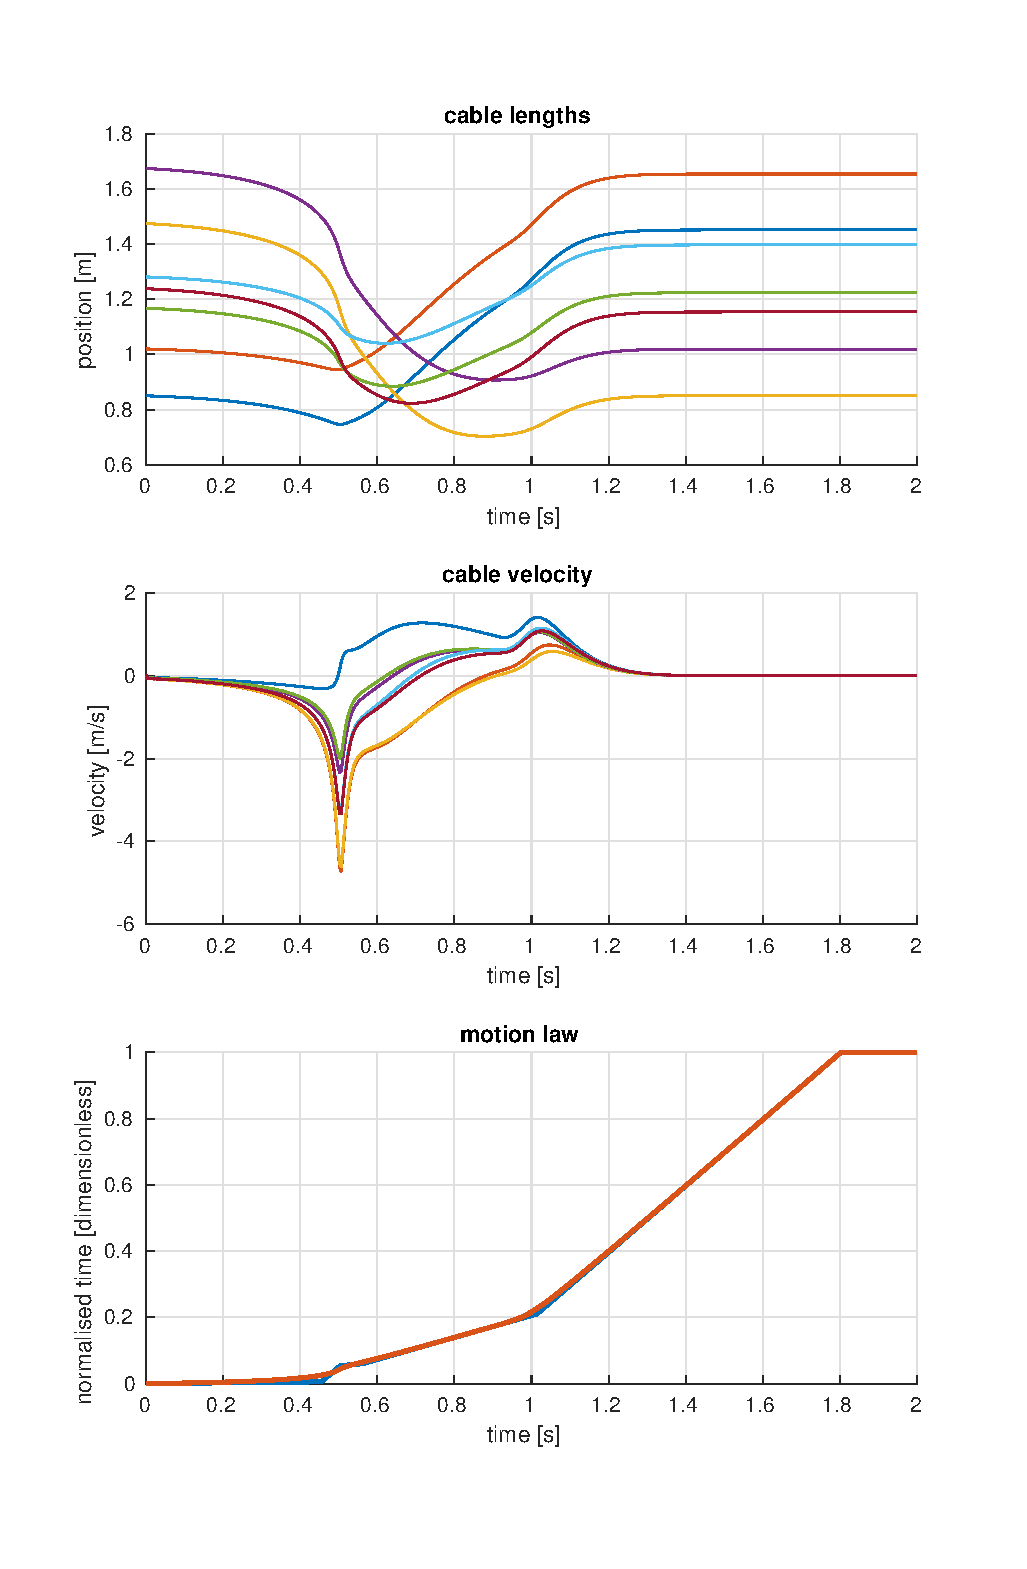
\includegraphics[width=\textwidth]{motion_law_deg_3}
			\caption{Motion Law with B-Spline\\\hspace{\textwidth} of Degree 3}
			\label{fig:motion_law_deg3}
		\end{minipage}%
		\begin{minipage}{0.5\columnwidth}
			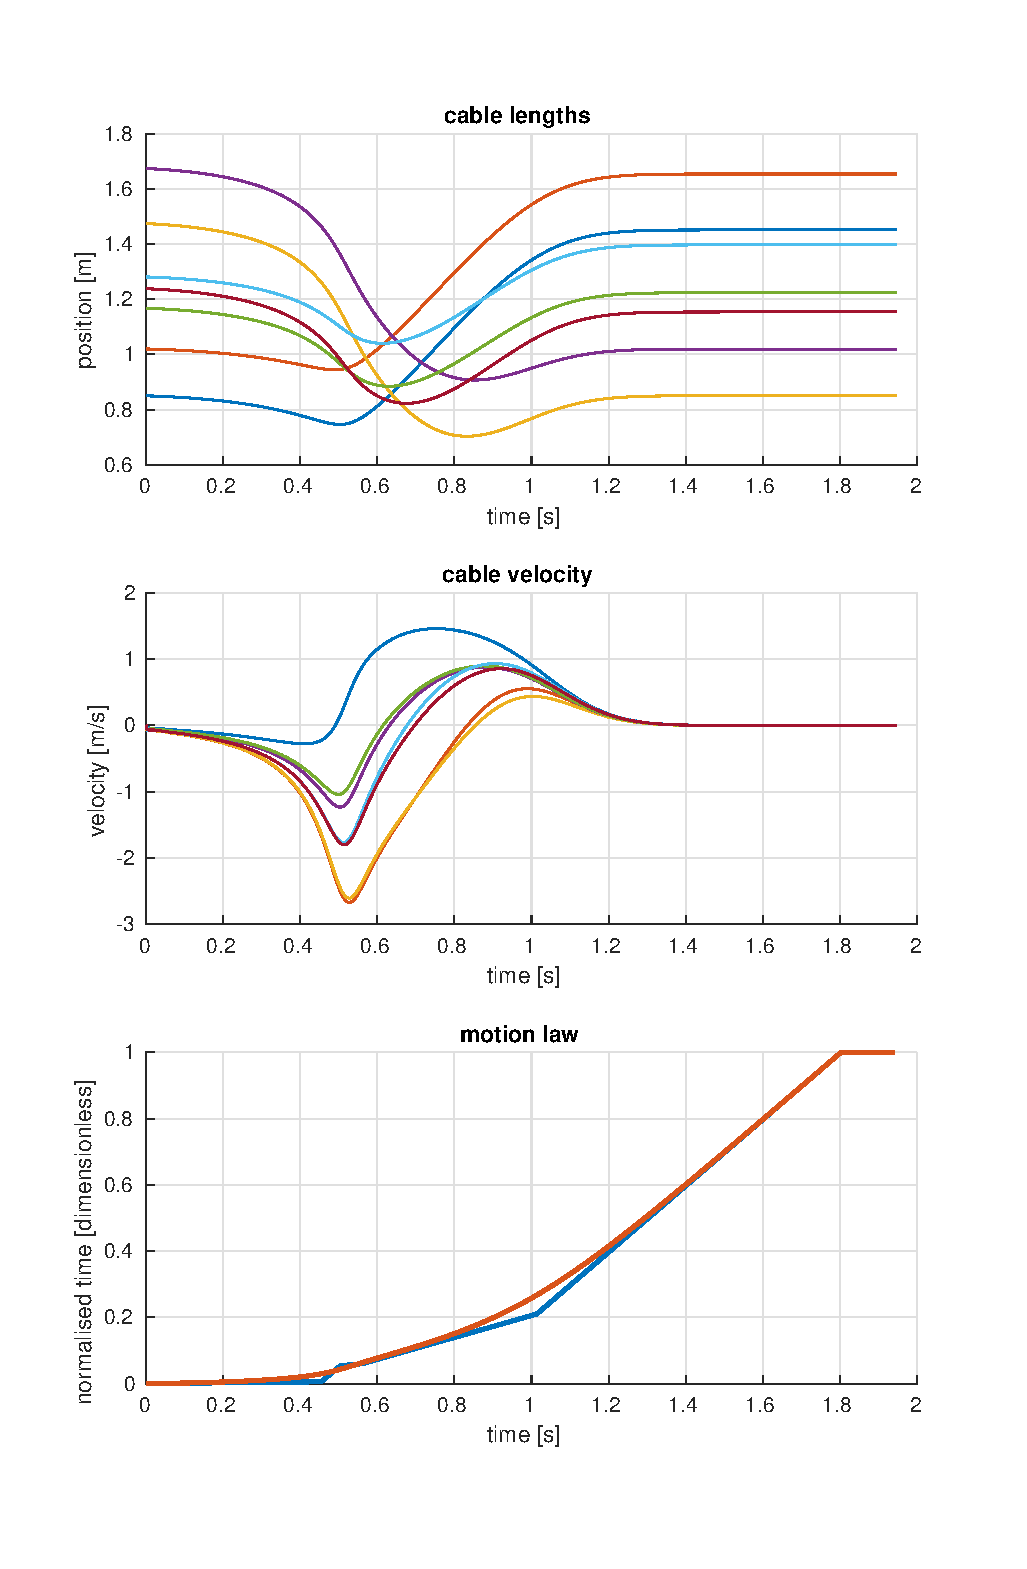
\includegraphics[width=\textwidth]{motion_law_deg_7}
			\caption{Motion Law with B-Spline\\\hspace{\textwidth} of Degree 7}
			\label{fig:motion_law_deg7}
		\end{minipage}
	\end{figure}
